\documentclass[10pt]{article}
\usepackage{enumitem}
\usepackage{listings}
\usepackage{underscore}
\usepackage[ddmmyyyy]{datetime}
\renewcommand{\dateseparator}{--}
\usepackage[bookmarks=true]{hyperref}
\usepackage[utf8]{inputenc}
\usepackage[english]{babel}
\usepackage{url}
\usepackage{graphicx}
\usepackage[labelfont=bf]{caption}

\newenvironment{enum}
{\begin{enumerate}[label*=\arabic*.][resume]}
{\end{enumerate}}

\hypersetup{
    pdftitle={Software Requirement Specification},    
    pdfauthor={Dakota Wessel},                     
    pdfsubject={TeX and LaTeX},                        
    pdfkeywords={TeX, LaTeX, graphics, images}, 
    colorlinks=true,       
    linkcolor=blue,       
    citecolor=black,       
    filecolor=black,        
    urlcolor=purple,        
    linktoc=page            
}
\def\myversion{1.0.4}
\date{}
\usepackage{hyperref}
\begin{document}

\begin{flushright}
    \rule{16cm}{5pt}\vskip1cm
    \begin{bfseries}
        \Huge{SOFTWARE REQUIREMENTS\\ SPECIFICATION}\\
        \vspace{1.0cm}
        for\\
        \vspace{1.0cm}
        Checkers\\
        \vspace{1.5cm}
        \LARGE{Version \myversion}\\
        \vspace{1.5cm}
        Prepared by:\\
    Adam Luong\\
    Benny Mai\\
    Dakota Wessel\\
    Jacky Zheng\\
    Tony Zhu\\
        \vspace{1.9cm}
        Group: \textbf{10}\\
        \vspace{1cm}
        \today\\
    \end{bfseries}
\end{flushright}

\tableofcontents

\section*{Revision History}

\begin{center}
    \begin{tabular}{|c|c|c|c|}
        \hline
        Name & Date & Reason For Changes & Version\\
        \hline
        1.0.0 & \formatdate{15}{10}{20} & Initial Setup & Dakota Wessel\\
        \hline
        1.0.1 & \formatdate{18}{10}{20} & Intro. and Use Cases & Benny Mai\\
        \hline
        1.0.2 & \formatdate{18}{10}{20} & Functional Requirements & Jacky Zheng\\
        \hline
        1.0.3 & \formatdate{18}{10}{20} & Nonfunctional Requirements & Adam Luong\\
        \hline
        1.0.4 & \formatdate{18}{10}{20} & Overall Description \& User Interface & Tony Zhu\\
        \hline
    \end{tabular}
\end{center}

\section{Introduction}

\subsection{Purpose of Document}
The goal of this document is to outline the requirement specifications of our web-based checkers game. 
This application will allow two users to connect and interact remotely, allowing them to play and chat. 
This document will cover the scope, objective, basic requirements, and goals for this application. 
After the application's high-level look, this document will dive deeper into topics like functional, 
non-functional, user interface, design, test cases, program usage, and references. 
This document will clearly explain to an engineer or end-user the overall implementation 
and goals of our application.

\subsection{Project Scope}
The main objective for documentation is to educate the reader about our Checkers application, 
its functionality, the technologies used, and outline the application requirements.

\subsection{Overview of Document}
The documentation will provide a clear explanation about which technologies we used, 
how we implemented them, and why we chose to use them. It will outline each component 
of our application. The flow starts with the functional requirements, non-functional requirements, 
user interface, and finished with lobbies, gameplay, and winning conditions, concluding with our references. 

\subsection{Background}

\subsubsection{History}

Throughout history, the game Checkers has been around, so the exact date for Checkers' 
invention is unknown. One of the earliest records of the game dates back to 3000 B.C in what 
is present-day Iraq. Later in Egypt, in 1400 B.C, the game was played using a 5 x 5 board \cite{historyCheckers}. 
However, the version of Checkers that we know of today was established in the mid-1500s by an English mathematician. 
Now the board game of checkers is cemented as one of the most popular board games of all time. 
\subsubsection{Game Rules}
    The rules provided are from the American Checker Federation \cite {checkersFoundation}.
    \begin{enumerate}
    \item Red always makes the first move.
    \item A player can forfeit at any time; as a result, the opponent wins.
    \end{enumerate}
\subsubsection{Moves} 
\begin{enumerate}
    \item A player may only move their own pieces.
    \item Normal Piece
        \subitem A normal piece may only move toward the other player's side of the board.
        \subitem A normal piece may move diagonally to the left or right to a vacant square in front of it.
        \subitem A normal piece may capture on the diagonal if there exists a vacant square one more diagonal position ahead.
            \subsubitem A piece may move again if there exists another piece to capture after making a capture.
    \item A King Piece moves the same as a normal piece but can move and capture backward.
    \item A King Piece may capture forward or backward.
    \item If a normal piece reaches the opposite edge of the board, it becomes a King Piece.
\end{enumerate}   

\subsubsection{Win Condition}
\begin{enumerate}
    \item When one player has no more pieces to move, the other player is the winner.
    \item If a player forfeits the match, the other player is conceded the winner.
\end{enumerate}

\subsection{Abstract}

Our goal is to create a document that will help a team member create an application, 
both client-side and server-side, that allows remote users to play checkers. The construction of this application will host one game of checkers to two users. 
\section{Overall Description}

\subsection{Product Perspective}

\indent \indent Checkers is a game meant to be played by two players on a 8x8 checkerboard with 12 dark pieces and 12 light pieces on opposing sides of the board. The pieces are placed on the dark checkered squares on the first 3 rows of each player's respective side. The objective of the game is to place the opposing player’s pieces in a position where the opposing player can no longer make any moves.

\indent The game is meant to be run on 2 computers/web browsers on a website(server). Each player will be able to connect to the server and have the board displayed to them on their web browser, each player's moves will be recorded by the server and then be sent to each player's browsers to accurately display the current board state. 

\begin{figure}[h!]
    \centering
    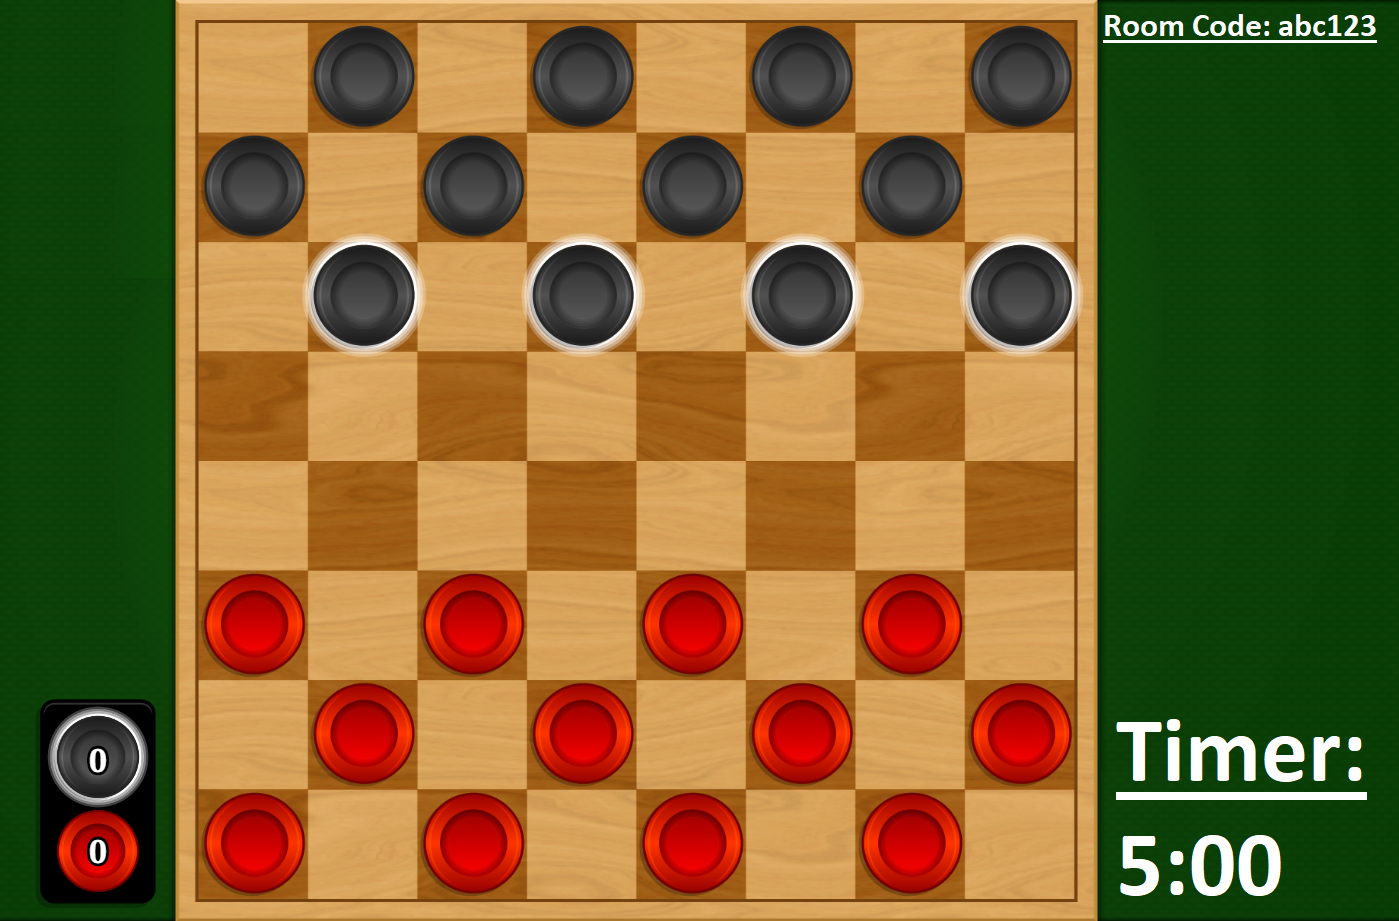
\includegraphics[width=8cm]{Mockup Game Screen.png}
    \caption{Mockup of the main game screen, board used from reference 3}
\end{figure}

\indent The game will display a top down view of the 2-D board as well as a timer and room code as seen in Figure 1. The room code will be used to match players with one another. Likewise the players will interact with the pieces displayed on the board with their mouse to perform moves.

\subsubsection{Web Browser/Computer Interface}
\indent \indent The users will only be interfacing with the game through a web browser. The browser will contain a menu to either create a game or join a game through a code. Likewise, it will also allow the players to move the pieces and also display the current board and time remaining per turn for to the users.

\subsection{Product Functions}

\begin{flushleft}
    {\large 2.2.1. Server Functionality:}
        {\begin{enumerate}
            \item The Server will perform the following:
            \begin{itemize}
                \item Remains running to allow users to connect to one another through web sessions
                \item The server will mediates gameplay, game sessions, and client interactions.
            \end{itemize}
        \end{enumerate}}
\end{flushleft}

\begin{flushleft}
    {\large 2.2.2. Web Browser/Client Functionality:}
        {\begin{enumerate}
            \item The Client will perform the following:
            \begin{itemize}
                \item Ability to create new game session with unique code
                \item Ability to connect to game sessions with unique code through server
                \item Update board based on data from server
            \end{itemize}    
    \end{enumerate}}
\end{flushleft}

\subsection{User Description}
The ideal users for Checkers would be 2 players 

\subsection{Assumptions and Dependencies}

\begin{flushleft}
    {\large 2.4.1. SQLite}
        \begin{itemize}
            \item The server will be using a SQLite database to hold all the data used to control the game of Checkers. Therefore, if SQLite were to cease support or no longer be available the team would have to restart development with a completely new database in order to proceed, which is not immpossible but will take significant amounts of time. The team assumes that SQLite will continue to work as intended.            
        \end{itemize}
\end{flushleft}

\begin{flushleft}
    {\large 2.4.2. Webserver}
        \begin{itemize}
            \item The team will be hosting the game on a webserver, as such if said webserver were to crash or become unavailable, the team would have to rehost the game on a new webserver. The team assumes that the webserver will stay online as intended.
        \end{itemize}
\end{flushleft}

\subsection{Requirements Apportioning}
\begin{figure}[h!]
    \begin{flushright}
        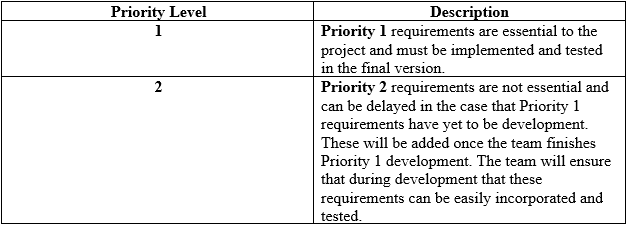
\includegraphics[width=13cm]{Priority Chart.png}
    \end{flushright}
\end{figure}
\pagebreak

\section{Functional Requirements}

\subsection{Client}

\begin{enumerate}[label*=R\arabic*.]
    \item Client - Server Interaction
    \begin{enumerate}[label*=\arabic*.]
        \item Client will automatically check to see if the game server is live given the set URL in the program.
        \item Client will not be able to join a lobby if no response is sent from the requested server URL.
        \item Client will be able to terminate itself from the server at any given moment.
        \item Client will be able to reconnect back to the lobby within 30 seconds, else they will receive a notification saying that the lobby has been closed and they are unable to rejoin due to the timeout period.
        \item Client should be able to distinguish themselves with a valid player name when they join a lobby.
    \end{enumerate}
\end{enumerate}

\subsubsection{Board State}

\begin{enumerate}[resume*]
    \item Board
    \begin{enumerate}[label*=\arabic*.]
        \item The clients will have a copy of the board for rendering purposes
        \item The board will update upon receiving a server update
    \end{enumerate}
\end{enumerate}

\subsection{Server}

\begin{enumerate}[resume*]
    \item Server should be able to be run constantly without crashing.
        \subitem Server will have a heartbeat function that will send an email to the developers if the server is down.
    \item Server - Client Interaction
    \begin{enumerate}[label*=\arabic*.]
        \item Server will be able to process client connection information to create a lobby.
        \item Server will keep track of clients and game sessions.
        \item On user timeout, wait a set amount of time.
            \subitem If not connected within that time, signal other client game has ended due to disconnected player.
        \item Server will validate moves before sending updated move to clients.
            \subitem On invalid move, signal client that move was invalid and to try again.
    \end{enumerate}
    \item Server - Lobby Interaction
    \begin{enumerate}[label*=\arabic*.]
        \item Server will first check that a port is open before assigning it to a lobby upon creation.
        \item Server will close the port assigned to a lobby when the game has been finished.
    \end{enumerate}
\end{enumerate}

\section{Non-Functional Requirements}

\subsection{Network Performance}

\begin{enumerate}[label*=N\arabic*.]
    \item Lag Management
	 \begin{enumerate}[label*=\arabic*.]
        \item Lag will be based off how stable the network connection of the computer the user is on. If network connection is table, there should be little to no lag. It should not negatively affect the game. Lag management will also be tested during the playtesting phase to ensure game quality.
	  \end{enumerate}
\end{enumerate}

\subsection{Host Operating System Requirements}

\begin{enumerate}[label*=S\arabic*.]
    \item Server
        \subitem Node.js to allow the client and the server to communicate through endpoints
        \subitem SQLite is used to store the generated key identifiers so that players can use that keycode to enter a room
    \item Client
        \subitem Support Desktop Browsers
            \subsubitem Google Chrome (latest stable version)
            \subsubitem Firefox (latest stable version)
            \subsubitem Microsoft Edge (latest stable version)
            \subsubitem Microsoft Internet Explorer 11
\end{enumerate}

\subsection{Accessibility}

\begin{enumerate}[label*=N\arabic*.]
    \item The application will be accessible through URL on the web browser
\end{enumerate}

\subsection{Playtesting}

\begin{enumerate}[label*=N\arabic*.]
    \item After the prototype is completed, the game will then undergo playtesting with approximately 8 people of any age, 4 being familiar with Checkers and 4 with the purpose of attempting to break the game. This way, it will test all aspects of the rules of Checkers and see if the game will run smoothly and correctly. It will also see if any moves that are not in the regulations of Checkers are being permitted within the game. Also it will see if players face little difficulty with the controls and understanding of our prototype. The game will be playtested near the end of Drexel Fall Quarter of 2020. After each playtesting session, the participants will fill out a form that helps answer the findings that we are testing for. The forms will be reviewed by the team. 
\end{enumerate}
\pagebreak
\section{User Interface}

\subsection{Menus}

\begin{figure}[h!]
    \centering
    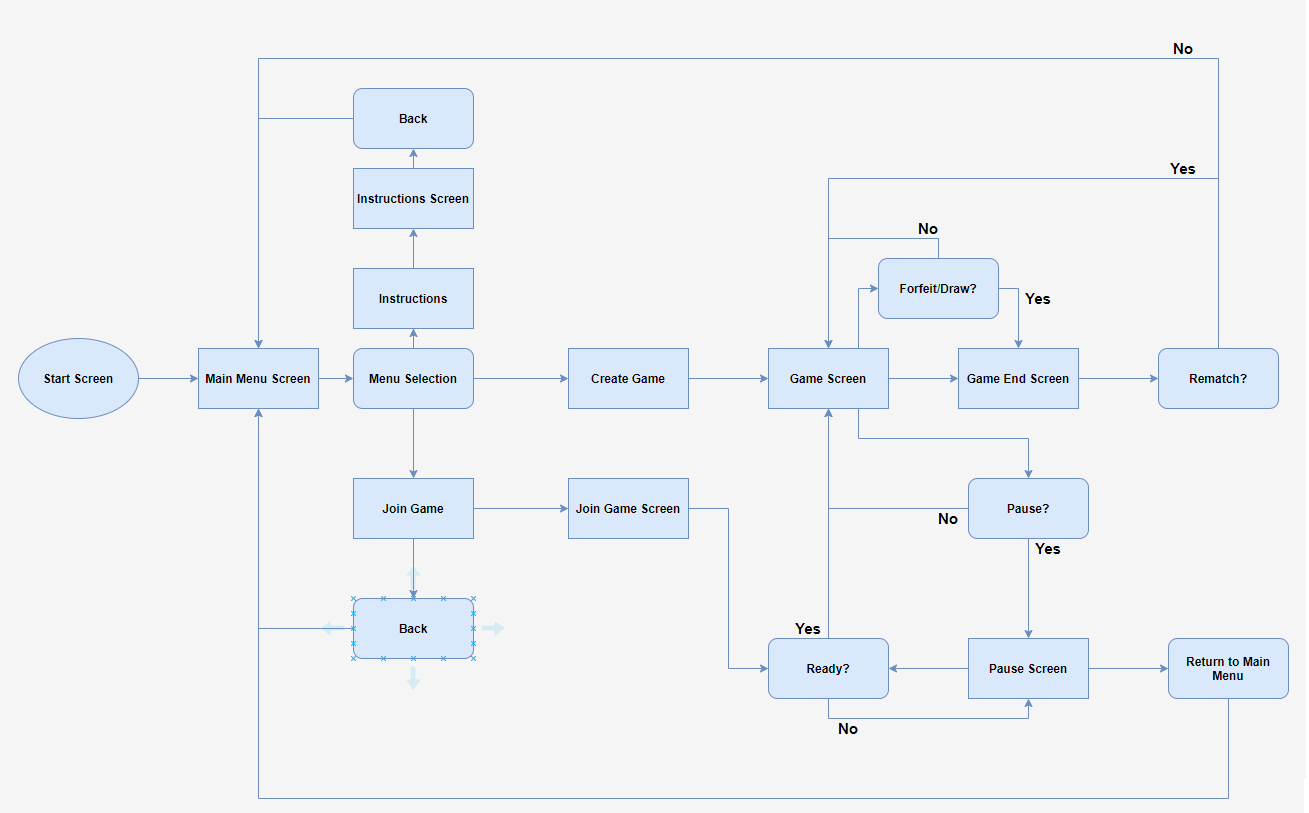
\includegraphics[width=16cm,scale=.5]{User Interface.png}
    \caption{Navigating menu screens on the client}
\end{figure}

\begin{enumerate}
\item Main Menu Screen - Contains 3 Buttons: Instructions, Create Game, Join Game
\begin{itemize}
    \item Create Game button: Generates room code, creates game instance and displays Game Screen. \textbf{Priority 1}
    \item Join Game button: Navigates to Join Game Screen. \textbf{Priority 1}
    \item Instructions button: Navigates to Instructions screen. \textbf{Priority 2}
\end{itemize}

\item Game Screen - Contains Checker Board with pieces, a player turn indicator (displays whose turn it is), Room Code, and a Timer (See Figure 1) along with 3 buttons: Draw, Forfeit, and Pause 
\begin{itemize}
    \item Room Code: Shows current room code - used by Player 2 to connect to game session. \textbf{Priority 1}
    \item Once game end condition is met (a player cannot make any more moves), Game End Screen will display \textbf{Priority 1}
    \item Players will control their pieces movements by interacting with the board using their mouse. \textbf{Priority 1}
    \item Turn indicator: Will display which players turn it is. Updates when a move on the board has been made by indicated player \textbf{Priority 1}
    \item Timer: Shows amount of time left for current player to make a move, if timer ends and no move is made then the current player will automatically lose and Game End Screen will display. \textbf{Priority 2}
    \item Draw button: Sends draw request to other player. \textbf{Priority 2}
    \item Forfeit button: Ends game and declares other player as winner. Navigates to Game End Screen. \textbf{Priority 2}
    \item Pause button: Sends pause request to other player. \textbf{Priority 2}
\end{itemize}

\item Game End Screen - Declares winner and a Rematch text that has 2 buttons under it: Yes or No
\begin{itemize}
    \item Winner will be declared on this screen \textbf{Priority 1}
    \item Yes button: Will display under "Rematch" text and navigate to Game Screen with new room code if selected. \textbf{Priority 2}
    \item No button: Will display under "Rematch" text and navigate to Main Menu Screen if selected. \textbf{Priority 2}
\end{itemize}

\item Instructions Screen - Contains game instructions and a back button
\begin{itemize}
    \item Displays instructions on how to connect or create game. As well as rules for the game Checkers. \textbf{Priority 2} 
    \item Back button: When clicked will return user back to Main Menu Screen. \textbf{Priority 2} 
\end{itemize}

\item Join Game Screen - Contains text box input that accepts a room code and a ready button
\begin{itemize}
    \item Room code text box will display and allow for alphanumeric input \textbf{Priority 1} 
    \item Ready button: When clicked, will validate inputted room code and navigate to Game Screen if the code is valid \textbf{Priority 1} 
\end{itemize}

\item Pause Screen: Will contain 3 buttons: Ready Player 1, Ready Player 2, Return to Main Menu
\begin{itemize}
    \item Ready Player 1 button: When clicked current player will be set as Player 1 and button unselectable from other players screen. When other player has clicked Ready Player 2 button both screens will navigate to the Game Screen. \textbf{Priority 2}
    \item Ready Player 2 button: When clicked current player will be set as Player 2 and button unselectable from other players screen. When other player has clicked Ready Player 1 button both screens will navigate to the Game Screen. \textbf{Priority 2}
    \item Return to Main Menu Butoon: When clicked the player will be taken to the Main Menu Screen. \textbf{Priority 2}
\end{itemize}

\end{enumerate}

\section{Standard Components}

\begin{itemize}
    \item Buttons: used for menu interations and navigation.
    \item Pieces: The pieces will be the basic playing pieces within gameplay.
    \item King Pieces: These pieces will behave identically to the regular pieces, but with additional movement options according to the rules of Checkers.
    \item Checkers Board: an 8x8 grid of alternating black and red tiles on which all pieces will be displayed in the gameplay.
\end{itemize}

\subsection{Program Usage}
\subsubsection{Gameplay}
\begin{enumerate}[label*=G\arabic*.]
	\item The match begins with an 8x8 grid with each tile alternating between black and red in color.
	\item One player is assigned the black pieces and the other red.
	\item Each player’s pieces start on opposite ends of the board, occupying every other space within the first three rows (for a total of 12 pieces for each player).
	\subitem See attached image for an example checkers setup:
	\begin{figure}[h!]
        \centering
        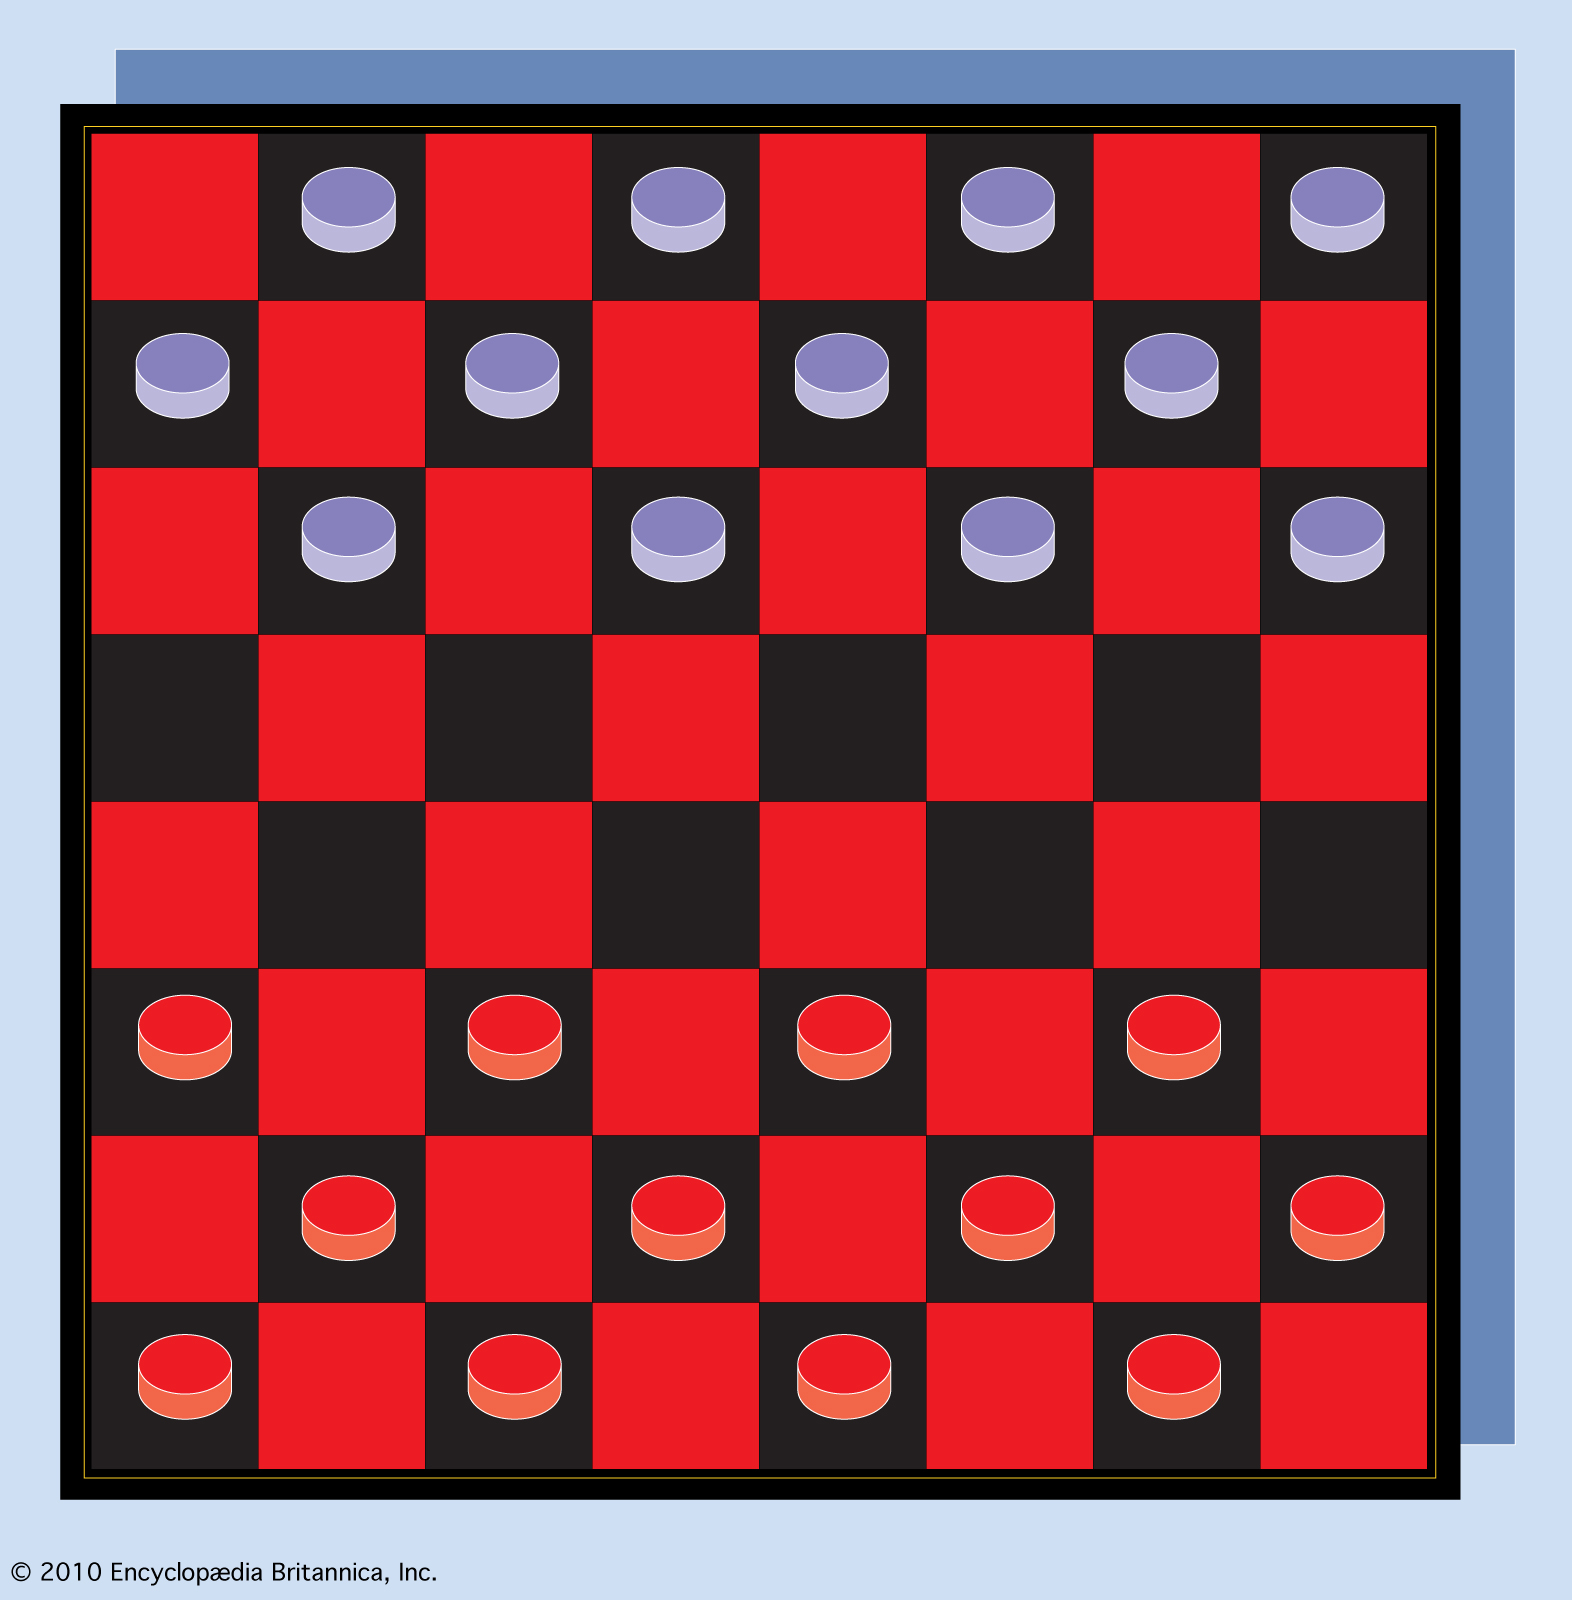
\includegraphics[width=8cm]{board.png}
        \caption{Example board, see reference 3}
    \end{figure}
	\item The black player starts the match by taking their turn.
	\item During each turn, the active player selects a piece of their own to move according to the following rules:
\begin{itemize}
    \item If the piece is bordering an enemy piece and there is a free space on the other side of that enemy piece, the piece must “jump” to the empty space, removing the enemy piece it moved over from the board
        \subitem Multiple jumps can be made in a single turn if the piece is in position to jump an additional enemy piece after completing a jump
    \item If the piece cannot jump, it may move diagonally one space to an unoccupied space
        \subitem If the piece is a non-king, it must move forward
        \subitem If the piece is a king, it can move in any direction
    \item A piece cannot jump over pieces of the same color as itself (friendly pieces)
    \item Two pieces cannot occupy the same space, regardless of color
\end{itemize}

\item When a non-king piece has reached the edge of the board opposite its color’s starting side, that piece will be crowned and turned into a king, allowing it to move in any direction.
\end{enumerate}
\subsubsection{Win Conditions}

\begin{enumerate}
    \item If player A has no more pieces, player B is the winner and vice versa.
    \item If player A disconnects, player B is the winner and vice versa.
\end{enumerate}


\begin{thebibliography}{9}

\bibitem{checkersFoundation}
  The American Checker Foundation,
  \textit{USA Checkers},
  https://www.usacheckers.com/,
  2019.

\bibitem{historyCheckers}
W.J. Rayment,
\textit{History of Checkers or Draughts},
http://www.indepthinfo.com/checkers/history.shtml,
2004.

\bibitem{Checkers}
Encyclopædia Britannica,
\textit{Checkers},
https://www.britannica.com/topic/checkers,
2018
\end{thebibliography}


\end{document}